\chapter{Toteutus}
\label{ch:toteutus}
Tässä osiossa käydään läpi kappaleessa \ref{ch:suunnittelu} suuniteltun ohjelman toteuttaminen. Toteutus alkaa yleiskuvalla sen komponenteista ja niiden toiminnasta. Yleiskuvan jälkeen pureudutaan ohjelman yksityiskohtiin kuten kirjastoihin ja niiden toimintaan. Lopuksi mietitään jatkokehitysideoita mitä olisi voinut lisätä, tehdä toisin ja mahdollisia puutteita.


\section{Yleiskuva}
\label{ch:rcb-sub-yleiskuva}
Työssä toteutetiin komentorivipohjainen ohjelma C-kielellä. Ohjelman tarkoitus oli tilata IED-laitteen viestit ja prosessoida ne JSON-muotoon RabbitMQ-palvelimelle. RabbitMQ:lta muut ohjelmat pystyivät tilaamaan JSON-viestejä. Kuvassa \ref{fig:rcb-sub-komponenttikaavio} on esitetty komponenttikaavio  toteutetusta ohjelmasta ja siihen käytetyistä kirjastoista. Toteutettu komponentti on kuvassa keskellä keltaisella ja nimelään rcb\_sub. Kuvasta voi nähdä miten eri komponentit ovat relaatiossa keskenään rcb\_sub-ohjelman kanssa. Kuvassa on myös esitetty IED-laite ja RabbitMQ-palvelin.

\begin{figure}[ht!]
	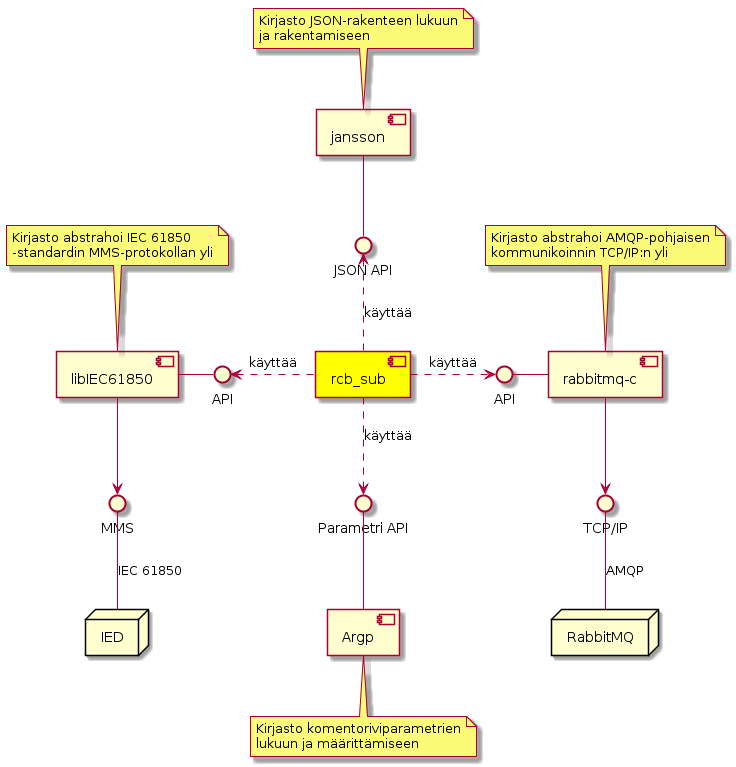
\includegraphics[width=1\textwidth]{pictures/rcb-sub-component-diagram.png}
	\caption{Toteutuksen komponenttikaavio sen osista ja relaatioista toisiinsa.}
	\label{fig:rcb-sub-komponenttikaavio}
\end{figure}

Toteutuksessa käytettiin seuraavia kirjastoja:
\begin{itemize}
	\item libiec61850,
	\item rabbitmq-c,
	\item jansson, ja
	\item Argp.
\end{itemize}
Kaikki käytetyt kirjastot on toteutettu C-kielellä, kuten rcb\_sub. Kirjastojen tarkoitus on abstrahoida jonkin asian käyttö ja tarjota käyttäjälle siitä helppokäyttöinen ja ymmärrettävä rajapinta. Rajapintaa käyttämällä kirjasto hoitaa matalan tason toiminnan ilman että kirjaston käyttäjän tarvitsee siitä välittää. Kirjasto libiec61850 abstrahoi IEC 61850 -standardin käyttöä ja hoitaa matalan tason MMS-protokollan kommunikoinnin \cite{libIEC61850-repo}. Samaa kirjastoa käytettiin ensimmäisessä demoversiossa (kappale \ref{ch:demoversio-ja-sen-toiminta}) ja kirjaston kerrosarkkitehtuuri oli esitetty kuvassa \ref{fig:libiec61850-layer-architecture}. Kuvassa \ref{fig:rcb-sub-komponenttikaavio} libiec61850 kommunikoi suoraan IED-laitteen kanssa MMS-protokollan yli. Kirjasto rabbitmq-c abstrahoi RabbitMQ-palvelimen käyttöä ja hoitaa matalan tason AMQP-pohjaisen kommunikoinnin \cite{rabbitmq-c-repo}. Toteutuksessa rabbitmq-c kommunikoi suoraan RabbitMQ-palvelimen kanssa. Kirjasto jansson abstrahoi JSON-rakenteiden lukua ja käsittelyä C-kielelle \cite{jansson-repo}. Kirjastoa käytettiin rakentamaan IED-laitteelta tulleesta viestistä JSON-muotoinen viesti. JSON-rakenne on nähtävissä liitteessä \ref{ch:report-json-format}. Kirjasto Argp auttaa ohjelman komentoriviparametrien määrittämisessä ja käsittelyssä \cite{argp-glibc-guide}. Kirjasto auttaa toteuttamaan ohjelmalle UNIX-tyyliset parametrit. Eli vaaditut parametrit ja vaihtoehtoiset lyhyet ja pitkä parametrit. Vaadituista parametreista esimerkiksi Linux:in komento \texttt{mv foo.txt bar.txt}, jossa foo.txt ja bar.txt ovat vaadittuja parametreja. Vaihtoehtoisista parametreista esimerkkinä pitkä muoto \texttt{-{}-bytes} ja lyhyt muoto \texttt{-b}. Lisäksi kirjasto lisää ohjelmaan automaattisesti Linux:ista käyttäjille tutut \texttt{-{}-help} ja \texttt{-{}-version} vaihtoehtoiset parametrit. Kommennolla \texttt{-{}-help} kirjasto tulostaa Linux:ilta tutun ohjelman aputeksin käyttäjälle, jossa on esitettu ohjelman kaikki parametrit ja niiden selitteet \cite{step-by-step-into-argp}.

Kuvassa \ref{fig:rcb-sub-sekvenssikaavio} on esitetty rcb\_sub-ohjelman sekvenssikaavio pääpiirteisestä toiminnasta. Toteutus noudattaa suurinpiirtein samoja periaatteita kuin demototeutus (kuva \ref{fig:sequence-diagram-report-subscription}). Tässä käydään läpi ohjelman pääpiirteinen toiminta ja sitä käydään tarkemmin läpi kappaleessa \ref{rcb-sub-toiminta}. Ensin ohjelman toiminta alkaa lukemalla ja annetut parametrit Argp-kirjastolla. Parametreissa tulee tiedot yhteyden muodostamiseen IED-laitteelle ja RabbitMQ-palvelimelle. Parametreissa on myös tiedot RCB-instansseista jotka halutaan IED:ltä tilata. Yhteyksien muodostamisen jälkeen jokainen parametrina annettu RCB käydään läpi silmukassa ja sen arvot ja datajoukon viitteet luetaan IED:ltä. Tämän jälkeen sisäkkäisessä silmukassa luetaan datajoukon viitteiden muuttujien spesifikaatiot (kohdat 11--12). Spesifikaatio antaa tiedot muuttujien pituudesta ja tyypistä. Näitä tietoja käytetään JSON-rakenteessa (esimerkkinä liiteessä \ref{ch:report-json-format} rivit 21--22). Tämän jälkeen tehdään toinen silmukka jossa jokainen RCB-instanssi tilataan ja niille asetetaan takaisinkutsufunktio (kohdat 13--16). Arvojen kirjoitushetkellä (kohta 15) RCB varataan ja se aloittaa viestien lähettämisen rcb\_sub-ohjelmalle. Jokaisen RCB:n kirjoituksen jälkeen ohjelma jää loputtomaan silmukkaan ja jää odottamaan viestejä vastaan. Viestin saapuessa asetettua takaisinkutsufunktiota kutsutaan ja jonka parametrina on saapunut viesti (kohta 17). Viesti muutetaan JSON-muotoon jansson-kirjastolla ja julkaistaan RabbitMQ-palvelimelle rabbitmq-c-kirjastolla (kohdat 17--22).

\begin{figure}[ht!]
	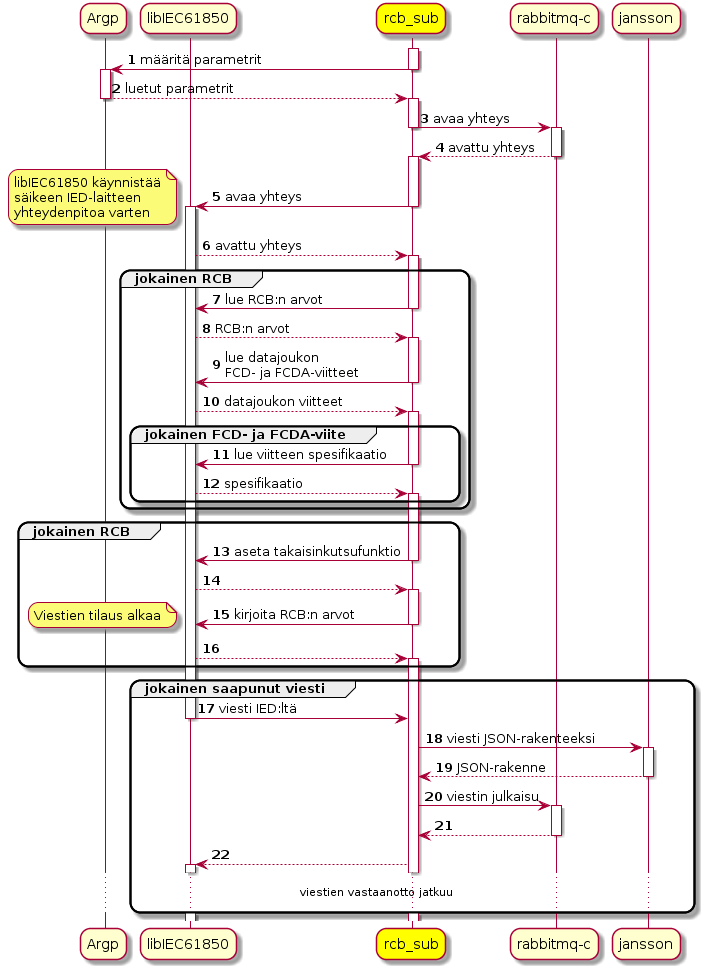
\includegraphics[width=1\textwidth]{pictures/rcb-sub-general-sd.png}
	\caption{Sekvenssikaavio rcb\_sub-ohjelman kokonaistoiminnasta.}
	\label{fig:rcb-sub-sekvenssikaavio}
\end{figure}


\section{Ohjelman toiminta}
\label{rcb-sub-toiminta}
Tulevissa kappaleissa käydään läpi yksityiskohtaisemmin rcb\_sub-ohjelman toimintaa, joka esiteltiin pääpiirteittäin kappaleessa \ref{ch:rcb-sub-yleiskuva}. Kappaleiden järjestys noudattaa kuvassa \ref{fig:rcb-sub-sekvenssikaavio} olevan sekvenssikaavion järjestystä. Toisin sanoen ohjelmaa käydään läpi tarkemmin siinä järjestyksessä jossa sen suoritus tapahtuu.


\subsection{Parametrisointi}
Ohjelma parametrisoitiin Argp-kirjastolla. Kirjasto tarjoaa rajapinnan komentoriviparametrien käsittelyyn ja määrittämiseen. Parametrien muodot ovat tuttut muista Linux-käyttöjärjestelmän parametreista ja samaa periaatetta käytettiin tässäkin ohjelmassa. Kirjasto myös lisäsi ohjelmaan automaattisesti aputekstin käyttäjää varten. Aputeksti sisältää tietoa ohjelman parametreista ja niiden selitteistä. Aputekstin pystyi ohjelmsata tulostamaan parametrilla \texttt{-{}-help}. Liitteessä \ref{ch:rcb-sub-help-output} on esitetty miltä toteutetun ohjelman aputeksti näyttyy. Liitteestä voi myös nähdä kaikki ohjelman käytettävät parametrit ja lyhyen selityksen mihin ja kuinka sitä käytetään.

Ohjelmiston parametrit voidaan ajatella koostuvan kolmesta eri ryhmästä. Ensin päätason vaihtoehtoiset parametrit \texttt{OPTIONS}. Pakolliset parametrit \texttt{EXCHANGE} ja \texttt{ROUTING\_KEY}. Viimeisenä n-kappaletta \texttt{RCB\_REF} ja \texttt{RCB\_OPTIONS} parametreja. Suurin osa \texttt{OPTION} parametreista on itsestäänselviä. Esimerkkinä \texttt{-{}-amqp-host}, joka kertoo AMQP-palvelimen IP-osoitteen. Tai \texttt{-{}-ied-host}, joka kertoo IED-laitteen IP-osoitteen johon yhdistetään. Parametrit \texttt{EXCHANGE} ja \texttt{ROUTING\_KEY} määrittävät nimet RabbitMQ-palvelimen vaihteelle ja reititysavaimelle. \texttt{RCB\_REF} määrittää viitteen tilattavaan RCB-instanssiin IED-laitteella. Tätä seuraava vaihtoehtoinen \texttt{RCB\_OPTIONS} määrittää parametrit edeltävälle RCB-instanssille, millä instanssi konfiguroidaan ennen tilausta. RCB-instansin parametri \texttt{RCB\_OPTIONS} määrittää käytetyt vaihtoehtoiset kentät (\texttt{-{}-opt-fields}), käytetyt liipaisimet (\texttt{-{}-trigger}) ja pyydetäänkö yleistä kyselyä ennen muita viestejä (\texttt{-{}-gi}). Liipaisimet ja vaihtoehtoiset kentät asetetaan numeerisella arvolla, jotka löytyvät myös aputekstistä (liite \ref{ch:rcb-sub-help-output}). Numeerisia arvoja voidaan summata yhteen asettamalla monta arvoa yhtä aikaa. Liipaisimien arvot vastaavat aikaisemmin kappaleessa \ref{ch:rcb-toiminta} esitettyjä arvoja. Vaihtoehtoisten kenttien arvot vastaavat aikaisemmin taulukossa \ref{tab:iec61850-optional-fields-definition} esitettyjä arvoja.

\subsection{Yhteyksien muodostus}
Parametrien luvun jälkeen ohjelma muodosti yhteydet ensin RabbitMQ-palvelimelle ja sen jälkeen IED-laitteelle. Kuvassa \ref{fig:rcb-sub-open-connections} on esitetty sekvenssikaavio mitä kirjaston funktioita ohjelma kutsuu missäkin järjestyksessä. Funktiot ja niiden parametrit voi tarkemmin tarkistaa kirjaston omasta dokumentaatiosta. Tämä kattaa yleiskuvasta \ref{fig:rcb-sub-sekvenssikaavio} kohdat 3--6. Vaikka kuvassa on esitetty että yhteydet avataan vain kerran. On ohjelma toteutettu niin, että niitä yritetään avata uudelleen jos yhteys katkeaa kesken suorituksen. Jos avaus ei onnistu, ohjelma kirjoittaa lokin tapahtuneesta ja odottaa hetken ennen uudelleen yritystä.

\begin{figure}[ht!]
	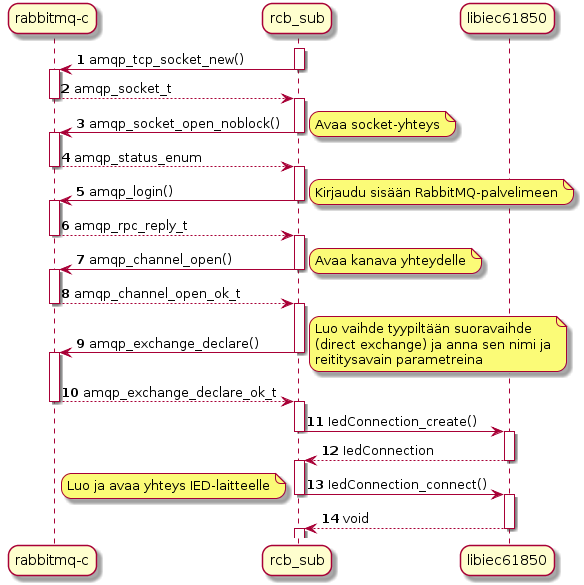
\includegraphics[width=1\textwidth]{pictures/rcb-sub-open-connections.png}
	\caption{Sekvenssikaavio kuinka rcb\_sub avaa yhteydet RabbitMQ-palvelimelle ja IED-laitteelle.}
	\label{fig:rcb-sub-open-connections}
\end{figure}

Yhteyden avauksen ja sisäänkirjautumisen jälkeen ohjelma avaa kanavan kohdassa 7--8. Kanava on yhteyden päälle avattu oma erillinen kommunikointiväylä, joka ei sotkeudu muihin kanaviin. Yhteen avattuun yhteyteen voi olla avattuna monta eri kanavaa. Kanavat mahdollistavat monen eri säikeen jakaa sama yhteys, ilman että tieto voisi vuotaa toiseen säikeeseen. Kohdassa 9 kutsutaan funktiota \texttt{amqp\_exchange\_declare()}. Funktio määrittää vaihteen tyyppiä suoravaihde RabbitMQ-palvelimelle. Suoravaihde käsiteltiin kappaleessa \ref{ch:direct-exchange}. Ohjelmaan ei toteutettu parametria vaihdetyypin määrittämiseen, koska katsottiin että suoravaihde on riittävä nykyisten vaatimusten täyttämisesksi. Tulevaisuudessa jos vaatimukset muuttuvat ja halutaan että käyttäjä voi valita käytettävän vaihdetyypin. Voidaan tämä toteuttaa lisäämällä ohjelmaan parametrit tätä varten.


\subsection{IED:n attribuuttien määritysten luku}
Yhteyksien muodostamisen jälkeen ohjelma käy läpi silmukassa jokaisen parametrina annetun RCB:n viitteen ja selvittää kaikkien parametrien specifikaatiot. Spesifikaatiotiedot sisältävät muuttujan tyypin ja sen koon. Kuvassa \ref{fig:rcb-sub-reading-specifications} on esitetty sekvenssikaavio kuinka rcb\_sub tämän tekee libiec61850-kirjastolla. Kuva vastaa yleiskuvassa \ref{fig:rcb-sub-sekvenssikaavio} kohtia 7--12.

\begin{figure}[ht!]
	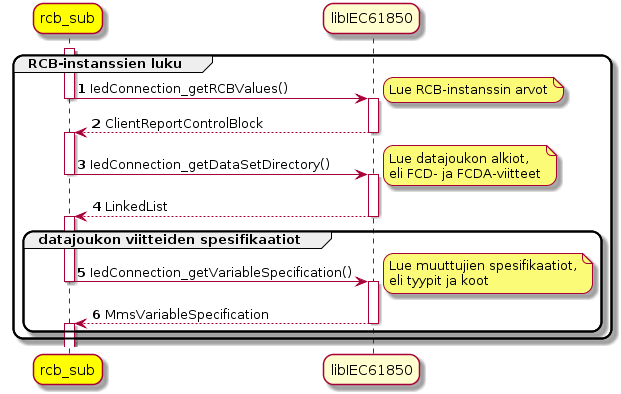
\includegraphics[width=1\textwidth]{pictures/rcb-sub-reading-specifications.png}
	\caption{Sekvenssikaavio kuinka rcb\_sub lukee RCB-instanssin arvot ja muuttujien spesifikaatiot.}
	\label{fig:rcb-sub-reading-specifications}
\end{figure}

Ensin RCB:sta luetaan sen tiedot IED-laitteelta. RCB:ltä saadaa tieto mihin datajoukkoon se on liitetty. Tätä käsiteltiin kappaleessa \ref{ch:rcb-toiminta} ja taulukossa \ref{tab:iec61850-brcb-class-definition} kenttä DatSet, joka kertoo käytetyn datajoukon viitteen. Tällä tiedolla ohjelma voi lukea datajoukon FCD- ja FCDA-viitteet. Tästä saadaan jokainen viite listassa, joka käydään läpi silmukassa kohdissa 5--6. Jokaiselle viitteelle luetaan sen spesifikaatio. Spesifikaatio rakenne sisältää sisäkkäisiä spesifikaatioita jos viite viittaa moneen muuttujaan IED-laitteen hierarkiassa. Tämä samalla periaatteella miten FCD- ja FCDA-viitteet viittaavaat moneen muuttujaan hierarkiassa alaspäin. Kuinka FCD- ja FCDA-viitteet toimivat käsiteltiin kappaleessa \ref{ch:fc-and-dataset}. Jokainen luettu viite tallennetaan ja niitä käytetään myöhemmin viestin kanssa JSON-rakenteessa. Esimerkkinä liitteessä \ref{ch:report-json-format} riveillä 21--22 tyyppi ja koko -tiedot.


\subsection{Viestien tilaus}
Ohjelman luettua kaikki muuttujien spesifikaatiot. Ohjelma tilaa silmukassa kaikki parametrina annetut RCB-instanssit. Kuvassa \ref{fig:rcb-sub-subscribe-reports} on esitetty sekvenssikaavio kuinka rcb\_sub tilaa RCB-instanssit libiec61850-kirjastolla. Kuvan vastaa yleiskuvassa \ref{fig:rcb-sub-sekvenssikaavio} kohtia 13--16.

\begin{figure}[ht!]
	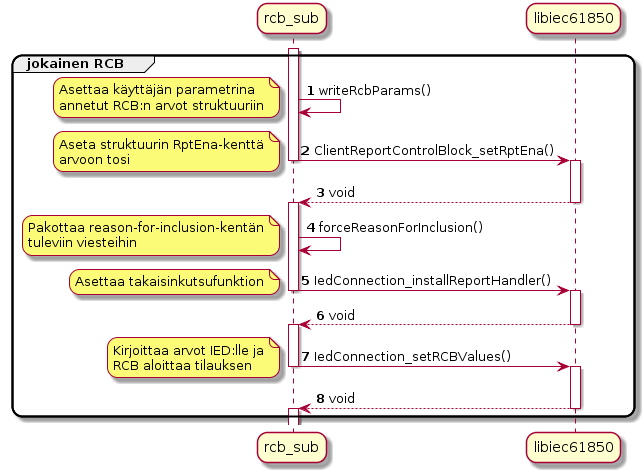
\includegraphics[width=1\textwidth]{pictures/rcb-sub-subscribe-reports.png}
	\caption{Sekvenssikaavio kuinka rcb\_sub tilaa RCB-instanssit.}
	\label{fig:rcb-sub-subscribe-reports}
\end{figure}

Ohjelma käsittelee libiec61850-kirjaston tarjoamaa stuktuuria ja kaikki arvot asetetaan siihen ennen oikeaa kirjoitusta. Ensin ohjelma asettaa kaikki käyttäjän antamat arvot struktuuriin. Kohdassa 2 asettaa asettaa RCB:n RptEna-kentän arvoksi tosi. Tämä kenttä varaa RCB-instanssin ja aloittaa tilauksen. Ohjelma pakottaa viestiin vaihtoehtoisen kentän reason-for-inclusion. Tätä kenttää tarvitaan, jotta aikaisemmin luetut spesifikaatiotiedot saadaan yhdistettyä saapuneeseen viestiin. Tämän jälkeen asetetaan takaisinkutsufunktio, jota kirjasto kutsuu kun viesti saapuu (kohta 5). Viimeisenä struktuurin arvot kirjoitetaan IED:llä olevalle RCB:lle. Tämä varaa RCB-instanssin tälle asiakkaakkalle ja aloittaa tilauksen. RCB tulee lähettämään viestejä ohjelmalle samalla kun silmukan muilla kierroksilla käsitellään tilaamattomia RCB-instansseja.


\subsection{JSON:nin muodostaminen ja julkaisu}
Viestin saapuessa libiec61580-kirjasto kutsui asetettua takaisinkutsufunktiota. Takaisinkutsufunktio muutti viestin JSON-muotoon ja lisäsi siihen aikaisemmin luetut muuttujien tyypit ja koot. Tämän jälkeen JSON-julkaistiin RabbitMQ-palvelimelle. Kuvissa \ref{fig:rcb-sub-report-to-json-1} ja \ref{fig:rcb-sub-report-to-json-2} on esitetty sekvenssikaaviolla kuinka ohjelma viestin muuttaa JSON:iksi ja julkaisee RabbitMQ:lle. Kuva \ref{fig:rcb-sub-report-to-json-1} vastaa yleiskuvan \ref{fig:rcb-sub-sekvenssikaavio} kohtia 17--19 ja kuva \ref{fig:rcb-sub-report-to-json-2} kohtia 20--22.

\begin{figure}[ht!]
	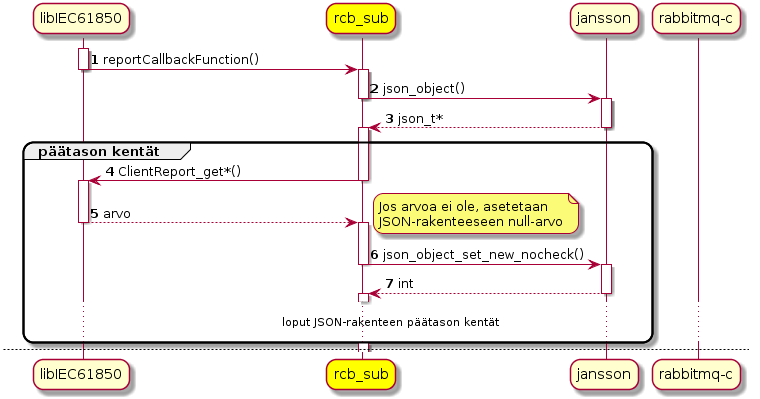
\includegraphics[width=1\textwidth]{pictures/rcb-sub-report-to-json.png}
	\caption{Sekvenssikaavio kuinka rcb\_sub muodostaa JSON:nin päätason kentät.}
	\label{fig:rcb-sub-report-to-json-1}
\end{figure}

Kuvassa \ref{fig:rcb-sub-report-to-json-1} alkaa kun libiec61850-kirjasto kutsuu takaisinkutsufunktiota. Funktiolle annetaan parametrina saapunut viesti. Tämän jälkeen ohjelma käy läpi viestin jokaisen päätason kentän ja lisää ne JSON-rakenteeseen. Osa viestin kentistä on vaihtoehtoisia riippuen mitä käyttäjä asetti \texttt{-{}-opt-fields} parametrilla. Jos arvoa viestissä ei ole, korvataan se null-arvolla JSON:iin. Esimerkkinä liiteessä \ref{ch:report-json-format} rivillä 4 oleva \texttt{confRevision} muuttuja, jonka arvo on null. Tämän jälkeen suoritus jatkuu kuvasta \ref{fig:rcb-sub-report-to-json-1} kuvaan \ref{fig:rcb-sub-report-to-json-2}.

\begin{figure}[ht!]
	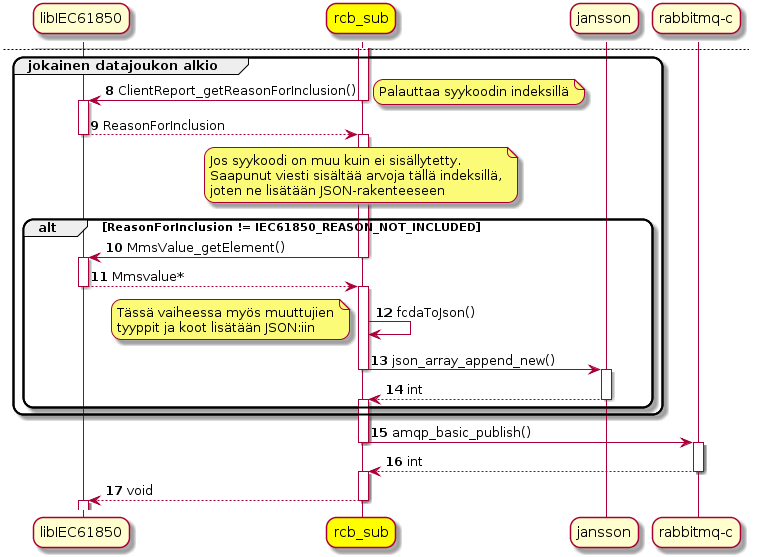
\includegraphics[width=1\textwidth]{pictures/rcb-sub-report-to-json_001.png}
	\caption{Sekvenssikaavio kuinka rcb\_sub lisää JSON:iin muuttujat viestistä.}
	\label{fig:rcb-sub-report-to-json-2}
\end{figure}

Päätason viestin kenttien jälkeen ohjelma käy läpi silmukassa viestin datajoukon indeksit (kuva \ref{fig:rcb-sub-report-to-json-2}. Viesti oikeasti sisältää vain ne datajoukon alkiot, mitkä sisältyivät viestiin. Ongelmana tässä on että viesti ei sisällä indeksiä tai tietoa siitä mikä datajoukon alkio on kyseessä mikä viestissä on. Jotta tästä saadaan tieto ohjelma pakottaa syykoodin päälle viestiin. Tämän avulla kun silmukassa käydään kaikki datajoukon indeksit läpi. Voidaan jokaiselle indeksille ensin kysyä syykoodi viestistä (kohdat 8--9). Jos datajoukon alkio ei ole viestissä, palauttaa kirjaston funktio \texttt{ClientReport\_getReasonForInclusion()} arvon \texttt{IEC61850\_REASON\_NOT\_INCLUDED}. Tätä tietoa voidaan käyttää löytämään oikea datajoukon indeksi. Jos datajoukon indeksi on viestissä, suoritetaan kohdat 10--14, muuten mennään seuraavaan indeksiin ja toistetaan kohdat 8--9. Datajoukon indeksi tarvitaan, jotta aiemmin luetut spesifikaatiot saadaan yhdistettyä muuttujiin arvojen kanssa. Datajoukon indeksillä, viestin arvoilla ja muuttujien tyypeillä ja koolla saadaan rakennettua loppuosa JSON-rakenteesta. Kuvassa \ref{fig:rcb-sub-report-to-json-2} oleva silmukka rakentaa liitteessä \ref{ch:report-json-format} olevan values-taulun alkaen riviltä 7. JSON:in sisempi values taulu (rivi 13) on lista FCD- tai FCDA-viitteen muuttujia mitä se viittaa arvoineen. Tämä taulukko muodostetaan kuvan \ref{fig:rcb-sub-report-to-json-2} kohdassa 12 funktiolla \texttt{fcdaToJson()} ja lisätään JSON:iin kohdassa 13. Lopuksi viesti lähetetään RabbitMQ-palvelimelle funktiolla \texttt{amqp\_basic\_publish()} ja takaisinkutsufunktio palaa (kohdat 15--17).

\section{Jatkokehitys}
Ohjelmaa jätettiin työssä pisteeseen missä se saavutti kaikki tarvittavat vaatimukset. Kuitenkin tulevaisuudessa ohjelmaa pystyy kehittämään lisää ja lisätä uusia ominaisuuksia tarpeen vaatiessa. Yksi tärkeä puute mikä jäi jatkokehitykseen työssä oli ohjelman testiympäristön pystytys ja sille yksikkötestit. C-ohjelmassa ei ole suoraan tukea yksikkötestien kirjoittamiseen. Ympäristön pystytys vaatii erillisen kirjaston projektin yhteyteen, millä yksikkötestit kirjoitetaan. Tämä jäi tulevaisuuden kehitystyöksi ja ei sisältynyt tähän työhön. Yksikkötestit ovat kuitenkin tärkeä osa ohjelman ylläpitoa ja toiminnan varmistamista muutosten jälkeen. Testit tullaan tarvitsemaan ennemmin tai myöhemmin.

Ohjelma toteutettiin nyt niin että se aina käyttää suoraa vaihdetyyppiä RabbitMQ-palvelimella. Tämä täytti työlle asetetut vaatimukset. Jos tulevaisuudessa tarvitaan joustavuutta, voidaan ohjelmaan tehdä muutoksia ja parametreja lisätä helposti lisämään toiminnallisuutta. Esimerkkinä käyttäjä voisi valita käytettävän vaihteen tyypin parametrilla.